%% %%%%%%%%%%%%%%%%%%%%%%%%%%%%%%%%%%%%%%%%%%%%%%%%%
%% Template for a conference paper, prepared for the
%% Food and Resource Economics Department - IFAS
%% UNIVERSITY OF FLORIDA
%% %%%%%%%%%%%%%%%%%%%%%%%%%%%%%%%%%%%%%%%%%%%%%%%%%
%% Version 1.0 // November 2019
%% %%%%%%%%%%%%%%%%%%%%%%%%%%%%%%%%%%%%%%%%%%%%%%%%%
%% Ariel Soto-Caro
%%  - asotocaro@ufl.edu
%%  - arielsotocaro@gmail.com
%% %%%%%%%%%%%%%%%%%%%%%%%%%%%%%%%%%%%%%%%%%%%%%%%%%
\documentclass[11pt]{article}
\usepackage{UF_FRED_paper_style}
\usepackage{fancyhdr}

\usepackage{lipsum}  %% Package to create dummy text (comment or erase before start)

\usepackage{listings}
\usepackage{listings-golang}
\usepackage{color}

\lstset{ % add your own preferences
    frame=single,
    basicstyle=\footnotesize,
    keywordstyle=\color{red},
    numbers=left,
    numbersep=5pt,
    showstringspaces=false, 
    stringstyle=\color{blue},
    tabsize=4,
    language=Golang % this is it !
}

%% ===============================================
%% Setting the line spacing (3 options: only pick one)
% \doublespacing
% \singlespacing
\onehalfspacing
%% ===============================================

\setlength{\droptitle}{-5em} %% Don't touch

\setlength{\parindent}{0pt}

% %%%%%%%%%%%%%%%%%%%%%%%%%%%%%%%%%%%%%%%%%%%%%%%%%%%%%%%%%%
% SET THE TITLE
% %%%%%%%%%%%%%%%%%%%%%%%%%%%%%%%%%%%%%%%%%%%%%%%%%%%%%%%%%%

% TITLE:
\title{PCP Project Go}


\pagestyle{fancy}
\fancyhf{}
\rhead{\today}
\lhead{Anna Huber \& Flavio Lazzarini}
\rfoot{\thepage}

% AUTHORS:
%\author{Anna Huber% Name author
% \and Flavio Lazzarini %% Email author 2
%    }
    
% DATE:
%\date{\today}

% %%%%%%%%%%%%%%%%%%%%%%%%%%%%%%%%%%%%%%%%%%%%%%%%%%%%%%%%%%
% %%%%%%%%%%%%%%%%%%%%%%%%%%%%%%%%%%%%%%%%%%%%%%%%%%%%%%%%%%
\begin{document}
% %%%%%%%%%%%%%%%%%%%%%%%%%%%%%%%%%%%%%%%%%%%%%%%%%%%%%%%%%%
% %%%%%%%%%%%%%%%%%%%%%%%%%%%%%%%%%%%%%%%%%%%%%%%%%%%%%%%%%%
% ABSTRACT
% %%%%%%%%%%%%%%%%%%%%%%%%%%%%%%%%%%%%%%%%%%%%%%%%%%%%%%%%%%
% %%%%%%%%%%%%%%%%%%%%%%%%%%%%%%%%%%%%%%%%%%%%%%%%%%%%%%%%%%
%{
%\maketitle
%}
\begin{center}
\textbf{\Large PCP Project Go}    
\end{center}

% %%%%%%%%%%%%%%%%%%%%%%%%%%%%%%%%%%%%%%%%%%%%%%%%%%%%%%%%%%
% %%%%%%%%%%%%%%%%%%%%%%%%%%%%%%%%%%%%%%%%%%%%%%%%%%%%%%%%%%
% BODY OF THE DOCUMENT
% %%%%%%%%%%%%%%%%%%%%%%%%%%%%%%%%%%%%%%%%%%%%%%%%%%%%%%%%%%
% %%%%%%%%%%%%%%%%%%%%%%%%%%%%%%%%%%%%%%%%%%%%%%%%%%%%%%%%%%

% --------------------
\section{Einleitung}
Go ist eine ausdrucksstarke, prägnante Programmiersprache, die 2012 von Google publiziert wurde. Mit Fokus auf paralleler Programmierung ermöglicht Go das Maximum aus Multi-Core Maschinen herauszuholen.
% --------------------

% --------------------
\section{Goroutines, Channels \& Select}
\subsection{Goroutines, Parallelität in Go}
Eine der grössten Stärken von Go ist die Parallelität. Mittels sogenannten Goroutines ist es in Go sehr simpel, Funktionen parallel zu starten. Die Go Dokumentation beschreibt Goroutines folgendermassen: \begin{quote}
``Eine Goroutine ist ein leichtgewichtiger Thread, welcher von der Go-Runtime verwaltet wird.'' -  \cite{ATourofG52:online}
\end{quote} 

Das Erstellen von solchen Threads ist mit dem Keyword \lstinline{go} möglich.
Per Default erstellt jede Go Applikation mindestens eine Goroutine, die \lstinline{main()} Goroutine. Da Goroutines leichtgewichtig sind, können Go Anwendungen tausende Goroutines besitzen. Das Codebeispiel concurrency.go enthält zeigt die Benutzung von Goroutines auf. (\cite{Anatomyo74:online})

\subsection{Channels, Kommunikation zwischen Goroutines}\label{subsec:channels}
Ein Channel ist eine typisierte Queue, welche die Datenübertragung zwischen verschiedenen Threads erlaubt. Channels synchronisieren die Übermittlung von Ressourcen zwischen Goroutines. Mit dem Keyword \lstinline{chan} können Channels erstellt werden. Dabei ist es wichtig zu beachten, dass Channels die Übertragung von nur einem Datentypen erlauben. Der Datentyp wird beim Erstellen des Channels angegeben.

\begin{lstlisting}[caption= Erstellen eines Channels]
c := make(chan int) //this channel sends and receives int values
\end{lstlisting}

Das Lesen und Schreiben eines Channels ist dank der Arrow-Syntax sehr intuitiv. 
\begin{lstlisting}[caption=Lesen und Schreiben von Channels]
c <- data //write
var readData <- c // read
\end{lstlisting}

\subsubsection{Unbuffered Channel}
Unbuffered Channels können nur einen Wert speichern. Damit Daten übertragen werden können, müssen dementsprechend beide Goroutines bereit sein. Wenn eine Goroutine auf einen unbuffered Channel schreiben will und keine Goroutine auf dessen Wert wartet, wird der Channel die schreibende Goroutine blockieren und in den Wartezustand versetzen. Das Gleiche gilt auch falls eine Goroutine aus dem Channel lesen will und keine Goroutine bereit ist um zu schreiben. Somit garantieren unbuffered Channels eine synchronisierte Kommunikation.

\subsubsection{Buffered Channel}
Buffered Channels können mehr als einen Wert speichern. Die Anzahl von Werten die ein Channel speichern kann, muss der Entwickler fest vorgeben. Wenn im Channel Platz für einen zusätzlichen Wert vorhanden ist, kann eine Goroutine, auch wenn keine lesende Goroutine vorhanden ist, in den Channel schreiben.  Solange Werte im buffered Channel vorhanden sind, können Goroutines diese Werte lesen, ohne blockiert zu werden. Falls eine Goroutine in einen vollen buffered Channel schreiben will, oder eine Goroutine aus einem leeren buffered Channel lesen will, wird die Goroutine blockiert. Buffered Channels agieren als FIFO Queues. (\cite{Guney2018})

\subsection{Select}
Manchmal kann es sinnvoll sein, die parallele Abarbeitung einer Funktion mehreren Funktionen zu übergeben. Beachten Sie das folgende Beispiel (der Code dazu ist im File select.go): Damit unsere Webapplikation skalierbar ist, laufen mehrere Instanzen unseres Webservers (in diesem Beispiel sind es 2). Unsere Go Applikation benutzt die Rest-API, welche von unserem Webserver angeboten wird. Uns spielt es keine Rolle welcher der beiden Server uns antwortet, Hauptsache ist, dass es der schnellere ist. 
In Go löst das \lstinline{select} Keyword dieses Problem. Wie es im Code Beispiel ersichtlich ist, sieht das Statement einem \lstinline{switch} ähnlich. In unserem Beispiel wird das \lstinline{select} solange blockieren, bis einer der beiden Channels einen Wert enthält. (\cite{Guney2018})
% --------------------

% --------------------
\section{Maps \& Slices}
% --------------------
\subsection{Maps}

Eine Map in Go ist nach dem Key-Value Prinzip aufgebaut und ist eine Sammlung dieser Key-Value Paare. Jeder Key ist dabei einzigartig. 
Der Default Nullwert einer Map in Go ist nil. Eine nil Map ist, ausgenommen davon, dass keine Elemente zu einer nil Map hinzugefügt werden können, äquivalent zu einer leeren Map.

Um eine vollständige Übersicht der Map Funktionen in go zu erhalten, konsultieren Sie das Beispiel im maps.go File im Code. (\cite{Maps:online})


\subsection{Slices}

Slices in Go sind den Arrays sehr nahe. Arrays werden in Go mit einer festen Grösse erstellt, wobei Slices diese Angabe nicht benötigen. Slices selbst speichern keine Daten, sondern erzeugen und zeigen auf ein Array, welches diese Daten enthält. Slices haben die Eigenschaften length und capacity. Length beschreibt die Länge des Slices und capacity die Anzahl Elemente, welche im unterliegenden Array gespeichert werden können.



\begin{figure}[htb]
  \centering
  \subfloat[Case 1]{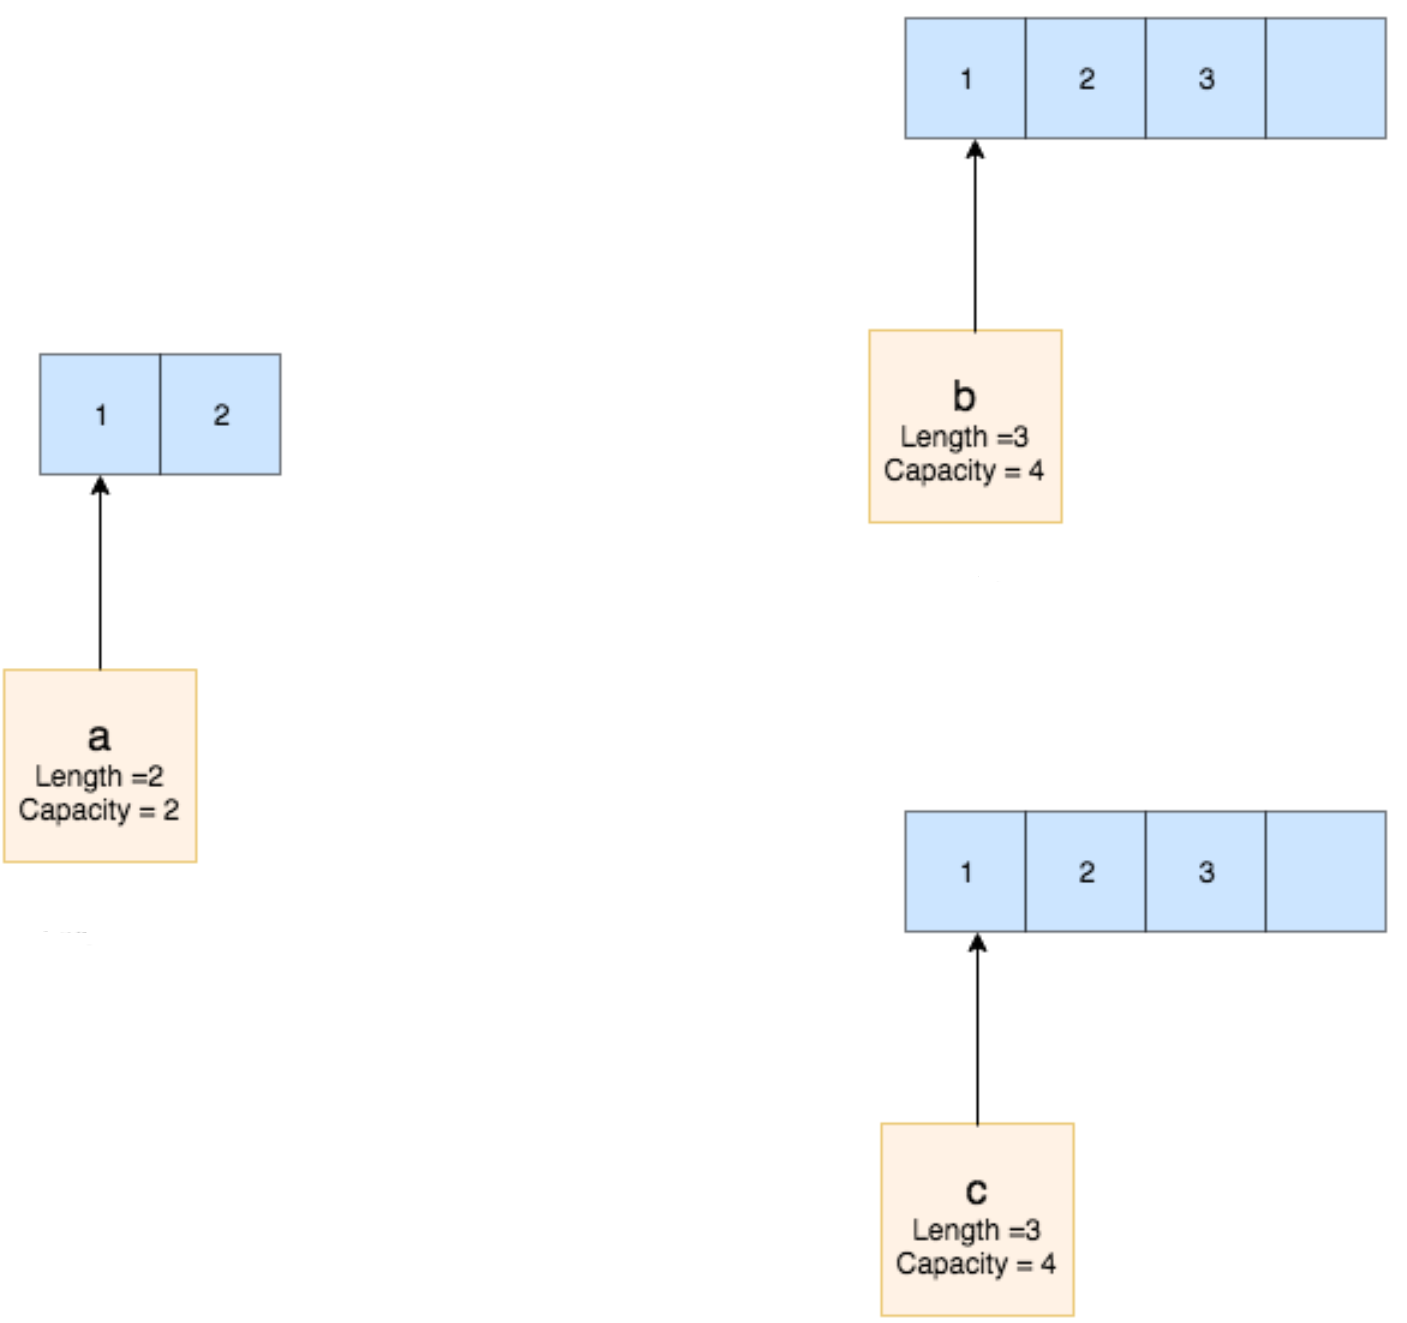
\includegraphics[width=0.35\textwidth]{figures/Slices Go 1.png}\label{fig:f1}}
  \hfill
  \subfloat[Case 2]{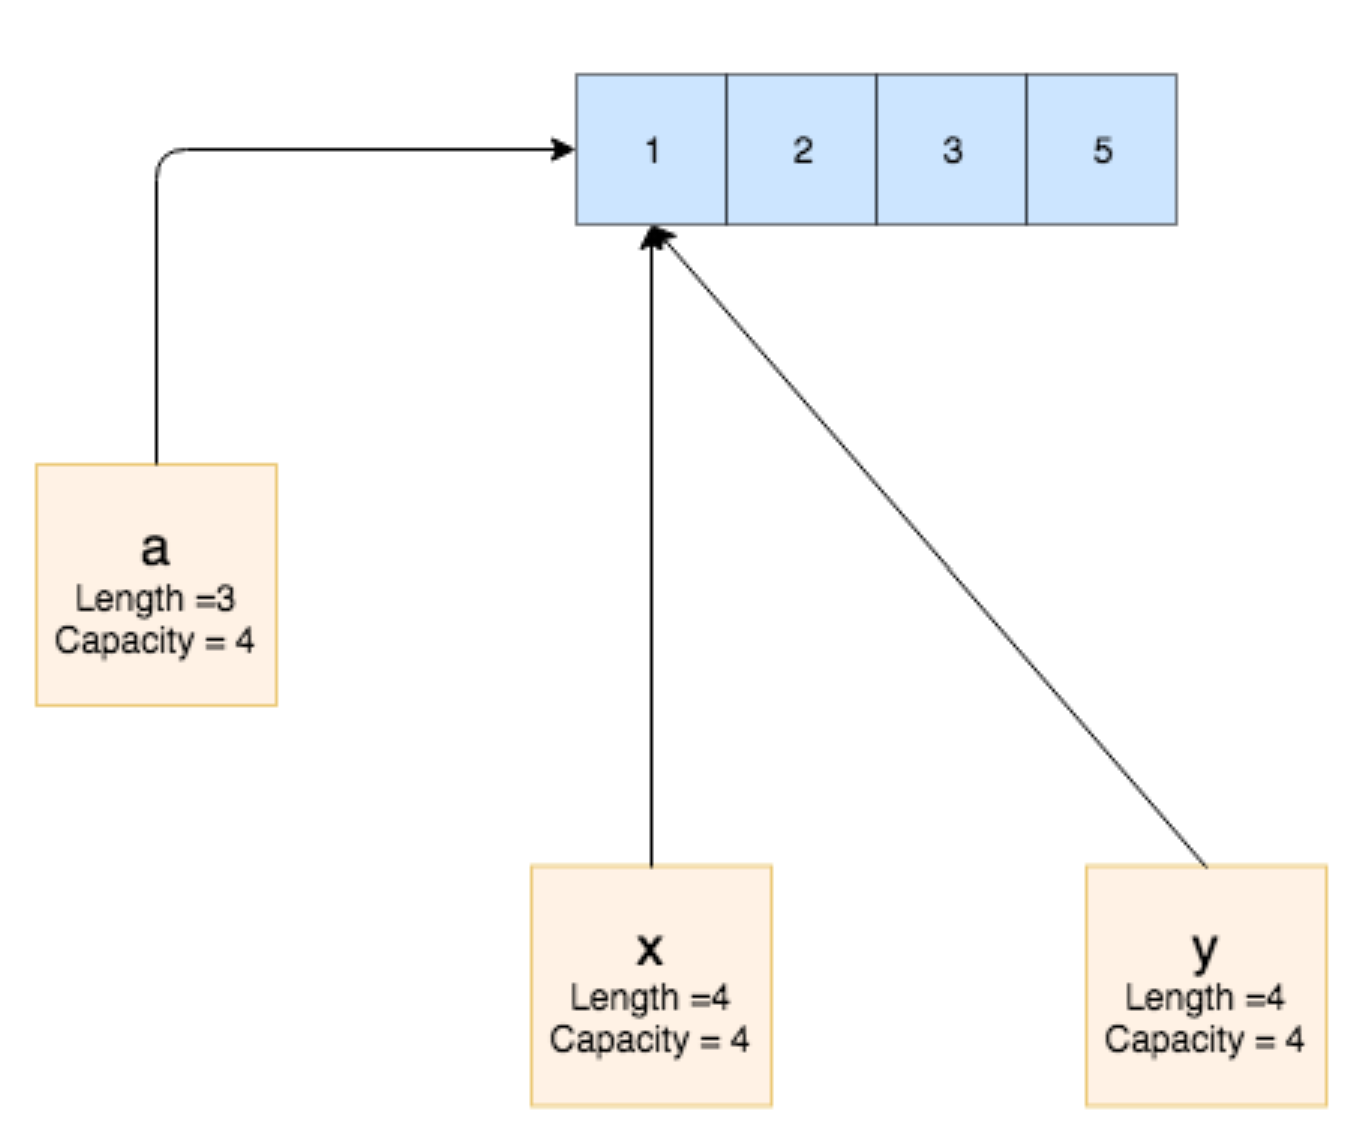
\includegraphics[width=0.35\textwidth]{figures/Slices Go.png}\label{fig:f2}}
  \caption{Slices  (\cite{Slices:medium})}
\end{figure}

Ein leeres Slice wird in Listing \ref{lst:Slices} auf Zeile 1 erstellt. Das Slice \lstinline{a} hat nach dem hinzufügen mit der Methode \lstinline{append} auf Zeile 2 eine Länge und capacity von 1. Auf Zeile 3 wird \lstinline{a} an eine neue Adresse mit capacity 2 alloziert. (Wenn die Länge eines Slices gleich der capacity ist und ein neues Element hinzugefügt wird, dann wird Memory mit der doppelten Kapazität des vorgängigen Memorys zum Slice alloziert.) Da auf Zeile 4 ein weiteres Element hinzugefügt wird, und length \lstinline{a} = capacity \lstinline{a} ist, wird ein neues Array mit Länge 4 (doppelte capacity zum vorherigen) erstellt. Wichtig hierbei ist, dass \lstinline{b} nicht auf das \lstinline{a} unterliegende Array zeigt, sondern auf das neu erstellte Array mit Länge 4. Das Slice \lstinline{b} hat daher Länge = 3 und capacity = 4.  Die capacity von \lstinline{a} bleibt 2. Auf Zeile 6 fügen wir nun ein neues Element zum Slice \lstinline{a} hinzu, was dazu führt, dass \lstinline{a} nun eine Länge von 3 und capacity von 4 hat.
Da sowohl das Slice \lstinline{x} als auch das Slice \lstinline{y} (Zeile 7 \& 8) auf das unter \lstinline{a} liegende Array zeigen, werden die durch y vorgenommenen Änderungen auch auf \lstinline{x} angewendet (Siehe Abbildung \ref{fig:f2}).
Slices können aber wie zum Beispiel in Python, auf bestehende Arrays erstellt werden. So können wir auf einfache Weise ein Slice \lstinline|s = a[1:2]| definieren. Damit folgt \lstinline|s = [2]| mit \lstinline|a = [1 2 3]|.
\begin{lstlisting}[caption=Slices in Go, label=lst:Slices]
	a := []int{}
	a = append(a, 1)    //a:  [1] 
	a = append(a, 2)    //a:  [1 2]
	b := append(a, 3)   //b:  [1 2 3] 
	c := append(a, 4)   //c:  [1 2 4]
	a = append(a, 3)    //a:  [1 2 3]
	x := append(a, 4)   //x:  [1 2 3 4] 
	y := append(a, 5)   //y:  [1 2 3 5]
	
	fmt.Println("x:", x) // x: [1 2 3 5]
\end{lstlisting}
(\cite{Slices:medium})






\section{Nominal vs. Structural Typing}
Jede typisierte Sprache besitzt ein Typesystem. In Typesystems kann zwischen Nominal Typing und Structural Typing unterschieden werden. In Nominal Typing Systemen sind zwei Variablen nur dann desselben Typs, wenn beide Typen den gleichen Namen besitzen. Dabei spielt es keine Rolle ob die Variablen dieselbe Struktur haben. Diese Typisierung ist von Programmiersprachen wie C oder Java bekannt. Dank Nominal Typing ist es unmöglich Variablen fälschlicherweise einem anderen Typen zuzuordnen, da diese Zuordnung nur über den Namen passiert. Die Typengleichheit wird in Structural Typing nicht anhand des Namens, sondern anhand der Struktur der Variablen definiert. Folgende Variablen wären somit Typengleich:
\begin{lstlisting}[caption=Beispiel von Structural Typing (Pseudo Code)]
struct human = {name, age}
struct dog = {name, age} //same type as human, they share the same attributes
\end{lstlisting}
Structural Typing ist somit flexibler als Nominal Typing.

\subsection{Typisierung in Go}
Go benutzt mehrheitlich Nominal Typing. Zum Beispiel sind folgende Typen nicht dieselben, da sie nicht denselben Namen besitzen:
\begin{lstlisting}[caption=Nominal Typing in Go]
type Human struct {
    name string 
    age int
}
type Dog struct {
    name string
    age int
}
\end{lstlisting}
Structural Typing wird in Go hingegen auf Methoden verwendet, um zu bestimmen, ob die Methode ein Interface implementiert. Nehmen wir an, wir hätten das folgende Interface gegeben:
\begin{lstlisting}[caption=Nominal Typing in Go]
type Being interface {
	Say() string
}

type Human struct {
	name string
}
\end{lstlisting}

Unser \lstinline{struct} muss nur eine Methode \lstinline{Say()} mit der gleichen Signatur wie die des Interfaces anbieten, um das Interface zu implementieren.
\begin{lstlisting}[caption=Implementation eines Interfaces]
type Human struct {
	name string
}

func (human Human) Say() string {
	return fmt.Sprintf("hello, my name is %s", human.name)
}
\end{lstlisting}

Beachten Sie folgende Methode, welche ein \lstinline{Being} als Parameter entgegen nimmt.
\begin{lstlisting}[caption=Verwenden eines Interfaces als Parameter]
func speak(being Being) {
	fmt.Println(being.Say())
}
\end{lstlisting}
Das interessante an Go ist, dass aufgrund des Structural Typings jedes struct, welches die Methode \lstinline{Say()} anbietet, als korrekter Parameter verwendet werden kann. Da die Methode \lstinline{Say()} public ist, können sogar structs aus externen Packages vom Typ \lstinline{Being} sein. Voraussetzung ist nur, dass sie eine Methode mit der Signatur \lstinline{func (type T) Say() string} besitzt. (\cite{Ducktypi27:online})


% --------------------
\section{The Go Memory Model}
% --------------------
Verschiedene Compiler oder Prozessoren führen Code-Optimierungen durch, indem sie die Ausführungsreihenfolge des Codes ändern. Dieses Verhalten nennt man Memory Ordering.

Das Go Memory Model spezifiziert, wie die Korrektheit eines Programmes eingehalten werden kann, wenn Goroutinen verwendet werden. Das heisst: Compiler oder Prozessoren dürfen Lese- und Schreibvorgänge innerhalb einer Goroutine nur dann umordnen, wenn diese die Semantik des Codes nicht verändert. Dafür wurden zwei Grundsätzliche Regeln festgelegt.

Das Lesen R einer Variablen v darf das Schreiben W von v dann sehen, wenn folgendes gilt:
 
\begin{enumerate}
    \item R geschieht nicht vor W.
    \item Es existiert kein anderes Schreiben W' nach v, welches nach W aber vor R geschieht.
\end{enumerate}

Um zu garantieren, dass das Lesen R der Variablen v ein spezifisches Schreiben W in v beobachtet, muss folgendes gelten:
\begin{enumerate}
    \item W geschieht vor R.
    \item Jedes andere Schreiben in v geschieht entweder vor W oder nach R.
\end{enumerate}

Damit diese Regeln von Go eingehalten werden können, müssen Synchronisationsmechanismen verwendet werden (siehe zum Beispiel Abschnitt \ref{subsec:channels}). (\cite{TheGoMem30:online})



% --------------------
\section{Package Management}
% --------------------
Für das Package Management wird in einem Go Projekt die Datei go.mod benötigt. In dieser Datei werden die im Projekt benötigten Packages und deren Versionen definiert.
Dieses File kann manuell oder in der CLI mit dem Befehl \lstinline[language=bash]{go mod init hslu/pcp/packer} erstellt werden.

Um dem Projekt neue Dependencies hinzuzufügen, benutzt man den Befehl \lstinline[language=bash]{go get} + url (beispielsweise \lstinline[language=bash]{go get github.com/google/uuid}).

Mit der Ausführung der Befehle \lstinline[language=bash]{go build} oder \lstinline[language=bash]{go test} werden die benötigten Dependencies automatisch heruntergeladen. Möchte man dies bereits vorher explizit ausführen, wird das mit \lstinline[language=bash]{go mod download} gemacht. Per default werden alle Packages unter \$GOPATH/pkg/mod gespeichert. 

Sowohl externe als auch interne Packages werden wie folgt importiert:

\begin{lstlisting}
import (
	"fmt"
	str "strings" // Package Alias
	"github.com/google/uuid"
	"hslu/pcp/packer/numbers"
	"hslu/pcp/packer/strings"
	"hslu/pcp/packer/strings/greeting" //import a nested package
)
\end{lstlisting}
\subsection{Sichtbarkeit von Funktionen und Konstanten}
In Go sind Funktionen und Konstanten  mit einem Grossbuchstaben startend automatisch public und mit einem Kleinbuchstaben startend automatisch private deklariert.

Die Sichtbarkeit einer Funktion oder Konstanten, wird automatisch mit deren Namensgebung definiert und es werden dazu keine Accessmodifiers benötigt.




% --------------------
\section{Fazit}
% --------------------

\subsection{Technisches Team-Fazit}
Go ist eine leistungsstarke Mischung aus low-level (z.B. C) und funktionalen Programmiersprachen (z.B. Lisp). Da der Go Compiler sehr restriktiv ist, ist es für Go-Neulinge einfach, korrekten Code zu schreiben. Aufgrund der eingebauten Funktionen bezüglich Nebenläufigkeit, eignet sich Go speziell für die Programmierung von APIs und Webanwendungen. Ausserdem wird Go sicherlich in den nächsten Jahren an Wichtigkeit gewinnen, da diese Sprache von Firmen wie Google, Docker oder Netflix verwendet wird.

\subsection{Persönliches Fazit Anna}
Go ist für mich eine interessante alternative zu Python. Durch den Aufwind den Go in den letzten paar Jahren erhalten hat, stehen inzwischen für AI und ML wichtige Packages, wie Tensorflow, sowohl in Python als auch in Go zur Verfügung. Ausserdem regelt Go mittels Goroutines und Channels die Funktionalitäten zur Parallelisierung von Code sehr elegant. Dadurch kann und wird Go auch in Cloud Computing verwendet. Zukünftig werde ich versuchen ein in Python geschriebenes Projekt in Go umzusetzen. 

\subsection{Persönliches Fazit Flavio}
Go wurde mit dem Hauptfokus auf Minimalismus entwickelt und hat dementsprechend kein grosses Set an eingebauten Funktionen. Dank dieser Eigenschaft ist Go einfach zu erlernen und zu lesen. Die Goroutines haben mir besonders gut gefallen. Sie ermöglichen das Programmieren von Nebenläufigkeit auf einfache und übersichtliche Weise. Die Verwendung von Interfaces gefällt mir hingegen nicht. Es ist sehr schwierig zu verstehen, von welchen Strukturen Interfaces geerbt werden. Aufgrund dessen, und da Go nur minimalistisches Error-Handling anbietet, eignet sich Go meiner Meinung nach nicht für komplexe Anwendungen. Ich würde Go jedoch gerne ausprobieren um einfache Web-Services zu schreiben.

% %%%%%%%%%%%%%%%%%%%%%%%%%%%%%%%%%%%%%%%%%%%%%%%%%%%%%%%%%%
% %%%%%%%%%%%%%%%%%%%%%%%%%%%%%%%%%%%%%%%%%%%%%%%%%%%%%%%%%%
% REFERENCES SECTION
% %%%%%%%%%%%%%%%%%%%%%%%%%%%%%%%%%%%%%%%%%%%%%%%%%%%%%%%%%%
% %%%%%%%%%%%%%%%%%%%%%%%%%%%%%%%%%%%%%%%%%%%%%%%%%%%%%%%%%%
\medskip

\bibliography{references.bib} 

\end{document}